\section{Statistics}

\begin{pgfplotslibrary}{statistics}
	A library which provides plot handlers for statistics.
\end{pgfplotslibrary}

\subsection{Box Plots}
\begingroup

\pgfkeysgetvalue{/pgfmanual/gray key prefixes}\oldgraykeyprefixes
\pgfkeys{
	/pdflinks/search key prefixes in/.add={}{,/pgfplots/boxplot/},
	/pgfmanual/gray key prefixes/.add={/pgfplots/boxplot/,}{},
}%

Box plots are visualizations for one--dimensional distributions. They provide a fast overview over characteristics of the distribution. Box plots are inherently one--dimensional; they only use a second axis to place multiple box plots next to each other.

\PGFPlots\ supports two related plot handlers: |boxplot| and |boxplot prepared|. 
	The |boxplot| handler takes a one--dimensional sample as input, computes the |median|, the |lower quartile|, the |upper quartile|, the |lower whisker| and the |upper whisker|, and visualizes the result using the |boxplot prepared| handler. The |boxplot prepared| handler expects all required values on input and visualizes them.

\subsubsection{Prepared Box Plots and Common Options}
The |boxplot prepared| handler is discussed first; all its customizations apply to |boxplot| as well.

\begin{plottype}[/pgfplots]{boxplot prepared=\textcolor{black}{\normalfont\marg{options with {\normalfont\texttt{boxplot/}} prefix}}}
	A |boxplot prepared| takes a couple of key--value pairs which describe the required statistics and additional information and a coordinate stream of outliers on input and draws a box plot.

\begin{codeexample}[]
\begin{tikzpicture}
\begin{axis}
	\addplot+[
		boxplot prepared={
			lower whisker=5,
			lower quartile=7,
			median=8.5,
			upper quartile=9.5,
			upper whisker=10,
		},
	]
		table[row sep=\\,y index=0] {
		data\\ 1\\ 3\\
	};
\end{axis}
\end{tikzpicture}
\end{codeexample}
	\noindent The previous example shows the main idea of |boxplot prepared|: each required quantity has to be provided explicitly using a key-value syntax. The following coordinate stream can be empty; all coordinates inside of it are considered to be outliers. They are drawn as scatter plot.

	A box plot produces two coordinates: one which belongs to the input data (for example |median|) and one which is only used for drawing purposes. Limits will be updated for both of them. While this is clear for the axis which shows the input data ($x$ in this example, see also |draw direction|), it should be noted that limits and scaling parameters for the other axis will be chosen just as for any other plot. The box's extend is a little bit less than one unit by default (compare |box extend|). As a consequence, would might need to adjust either the limits or the scaling parameters for the remaining axis:
\begin{codeexample}[]
\begin{tikzpicture}
\begin{axis}[
		y=1.5cm,
	]
\addplot+[
	boxplot prepared={
		lower whisker=5,
		lower quartile=7,
		median=8.5,
		upper quartile=9.5,
		upper whisker=10,
	},
]
	table[row sep=\\,y index=0] {
	data\\ 1\\ 3\\
};
\end{axis}
\end{tikzpicture}
\end{codeexample}
\end{plottype}

	If you place multiple blots with handler |boxplot prepared| into the same axis, they will automatically be placed next to each other by means of the default value of |draw position|:


\begin{pgfplotskey}{boxplot/draw position=\marg{axis unit to place box} (initially 1+\textbackslash plotnumofactualtype)}
	The |draw position| key determines how to choose the position of the box plot, i.e.\ the axis unit which is free to choose.

	The initial configuration places the first box plot at $y=1$ and all following ones at the next integer numbers.
\begin{codeexample}[]
\begin{tikzpicture}
\begin{axis}
\addplot+[
	boxplot prepared={
		lower whisker=42, lower quartile=45,
		median=47,
		upper quartile=47.5, upper whisker=48,
	},
]
	table[row sep=\\,y index=0] { 40\\ 34\\ 56\\ };

\addplot+[
	boxplot prepared={
		lower whisker=36, lower quartile=39,
		median=40,
		upper quartile=41, upper whisker=43,
	},
]
	% no outliers:
	coordinates {};

\addplot+[
	boxplot prepared={
		lower whisker=41, lower quartile=44,
		median=45,        
		upper quartile=46, upper whisker=47,
	},
]
	coordinates {(0,35) (0,55)};
\end{axis}
\end{tikzpicture}
\end{codeexample}
	The preceding example shows three box plots in the same axis. Note that they have been aligned using the default setting.

	The fact that the first $N$ |boxplot| (or the equivalent |boxplot prepared|) are placed at the coordinates $1,2,3, \dotsc,N$ makes it simple to assign tick labels: either use |ytick=data| or |ytick=1,2,3| combined with |yticklabels|:
\begin{codeexample}[]
\begin{tikzpicture}
\begin{axis}[
	ytick={1,2,3},
	yticklabels={Group A, Group B, Group C},
]
	\addplot+[
		boxplot prepared={
			lower whisker=42, lower quartile=45,
			median=47,
			upper quartile=47.5, upper whisker=48,
		},
	]
		table[row sep=\\,y index=0] { 40\\ 34\\ 56\\ };

	\addplot+[
		boxplot prepared={
			lower whisker=36, lower quartile=39,
			median=40,
			upper quartile=41, upper whisker=43,
		},
	]
		coordinates {};

	\addplot+[
		boxplot prepared={
			lower whisker=41, lower quartile=44,
			median=45,
			upper quartile=46, upper whisker=47,
		},
	]
		coordinates {(0,35) (0,55)};
\end{axis}
\end{tikzpicture}
\end{codeexample}

\noindent
	The |draw position| may be read from some input table using |draw position=\thisrow|\meta{colname}. In this case, the last encountered data row will be used (this remark is, of course, only useful if a data stream is present).
\end{pgfplotskey}

\noindent
	The preceeding examples read their outlier data streams from the $y$ coordinate of the input streams: for |\addplot table|, we have explicitly said |y index=0| and for |\addplot coordinates|, we have used |(0,35) (0,55)| where the $x$ components are ignored. This default can be changed using the |boxplot/data| key.
\begin{pgfplotskey}{boxplot/data=\marg{expression} (initially y)}
		Tells |boxplot| how to get its data. 
		The common idea is to provide a mathematical \meta{expression} which depends on data supplied by the |\addplot| statement. For example, if you have |\addplot expression|, the \meta{expression} may depend upon |x|, |y| or |z|. In case of an |\addplot table| input routine, the \meta{expression} can employ |\thisrow|\marg{colname} to access the currently active table row in the designated column.
		
		It is also possible to avoid invocations of the math parser. Use \declareandlabel{boxplot/data value}|=|\marg{value} instead to do so. Here, \meta{value} should be of a numeric constant.

		The initial configuration employs what would usually become the final |y| coordinate as input (to be more precise, the initial value is |data value=\pgfkeysvalueof{/data point/y}|).
\end{pgfplotskey}


\begin{pgfplotskeylist}{%
	boxplot/lower whisker=\marg{value} (initially auto),
	boxplot/lower quartile=\marg{value} (initially auto),
	boxplot/median=\marg{value} (initially auto),
	boxplot/upper quartile=\marg{value} (initially auto),
	boxplot/upper whisker=\marg{value} (initially auto),
	boxplot/average=\marg{value} (initially empty)%
}
	These keys constitute the supported statistics. Typically, a box plot uses each of them except for |average|.

	Any numeric value for \meta{value} will be used as-is. This holds for both |boxplot prepared| and |boxplot|.

	An empty \meta{value} disables the respective key: its associated visualization will be omitted. This is the default for |average|.

	The value |auto| tells \PGFPlots\ to include the statistics in the automatic computation applied by |boxplot|. It is irrelevant for |boxplot prepared| (where it is essentially the same as an empty \meta{value}).


	The definition of the values is as follows. Assume that we have a given sample of a distribution, say $x_1,\dotsc,x_N$, and assume that the values are sorted, $x_1 < \dotsb < x_N$ (which is not a requirement for |boxplot|, by the way). For any real number $p$ with $0\le p\le1$, the ``$p$--quantile'' (or $p$--percentage) is defined as
	\[
	x_p :=
	\begin{cases}
	 	x_{N \cdot p} & \text{if $N \cdot p$ is an integer number}\\
		\frac{1}{2} (x_{\lfloor N p \rfloor} + x_{\lceil N \cdot p \rceil}) & \text{if $N \cdot p$ is not an integer.}
	\end{cases}
	\]
	FIXME : this is not as in text--books! BUG in the computation!?
	
	|median| is the $0.5$--quantile of the input data: half of the points are less and half of the points are larger than the median.

	|lower quartile| is the $0.25$--quantile of the input data.

	|upper quartile| is the $0.75$--quartile of the input data.

	|lower whisker| is the smallest data value which is larger than |lower quartile|$ -1.5 \cdot \text{IQR}$ where $\text{IQR}$ is the ``inter--quartile--range'', i.e. the difference between |upper quartile| and |lower quartile|.

	|upper whisker| is the largest data value which is smaller than |upper quartile|$+1.5 \cdot \text{IQR}$.
	
	|average| is the sample average. It is omitted by |boxplot| in its default configuration. Set it to |auto| to enable its auto-computation.
\end{pgfplotskeylist}

\begin{pgfplotskey}{boxplot/draw direction=\mchoice{x,y} (initially x)}
	Since |boxplot| is inherently one--dimensional, it can be visualized along the $x$ or the $y$ axis.

	The default configuration uses the $x$ direction as seen above. 

	The alternative choice $y$ lets the boxes and their whiskers extend along the $y$~axis and stacks multiple box plots along the $x$ axis:

\begin{codeexample}[]
\begin{tikzpicture}
\begin{axis}[
	boxplot/draw direction=y,
	axis y line=none,
	axis x line*=bottom,
	xtick={1,2,3},
	xticklabels={Group A, Group B, Group C},
]
\addplot+[
	boxplot prepared={
		lower whisker=42, lower quartile=45,
		median=47,
		upper quartile=47.5, upper whisker=48,
	},
]
	table[row sep=\\,y index=0] { 40\\ 34\\ 56\\ };

\addplot+[
	boxplot prepared={
		lower whisker=36, lower quartile=39,
		median=40,
		upper quartile=41, upper whisker=43,
	},
]
	coordinates {};

\addplot+[
	boxplot prepared={
		lower whisker=41, lower quartile=44,
		median=45,
		upper quartile=46, upper whisker=47,
	},
]
	coordinates {(0,35) (0,55)};
\end{axis}
\end{tikzpicture}
\end{codeexample}
\end{pgfplotskey}

\begin{pgfplotskey}{boxplot/variable width=\mchoice{true,false} (initially false)}
	If enabled, the |box extend| will be scaled according to the |sample size| relative to all other |boxplot| or |boxplot prepared| within the same axis.

	FIXME: docs
\end{pgfplotskey}

\begin{pgfplotskey}{boxplot/sample size=\marg{number} (initially auto)}
	The number of samples used to derive the statistics. This number is used if |variable width=true|.
\end{pgfplotskey}

\begin{pgfplotskeylist}{%
	boxplot/sample size min=\marg{min sample size of group} (initially empty),
	boxplot/sample size max=\marg{max sample size of group} (initially empty)%
}
	This is part of the |variable width| scaling: it is used to determine the |box extend| relative to all other box plots of the same group. It fixes the range.

	FIXME: docs
\end{pgfplotskeylist}

\begin{pgfplotskey}{boxplot/variable width min=\marg{factor for the box width minimal size} (initially 0.2)}
	FIXME : docs
\end{pgfplotskey}

\begin{pgfplotskey}{boxplot/box extend=\marg{axis unit for box extension} (initially 0.8)}
	FIXME: docs
\end{pgfplotskey}

\begin{pgfplotskey}{boxplot/whisker extend=\marg{axis unit for whisker extension} (initially \textbackslash pgfkeysvalueof\{/pgfplots/boxplot/box extend\}*0.8)}
	FIXME: docs
\end{pgfplotskey}


\begin{pgfplotskey}{boxplot/draw relative anchor=\marg{number between $0$ and $1$} (initially 0.5)}
	FIXME : docs
\end{pgfplotskey}

\subsubsection{Analyzing Samples Automatically}
\begingroup
% this here seems to fail with gray key prefix:
\pgfkeyslet{/pgfmanual/gray key prefixes}\oldgraykeyprefixes

\begin{plottype}[/pgfplots]{boxplot=\textcolor{black}{\normalfont\marg{options with {\normalfont\texttt{boxplot/}} prefix}}}
	The |boxplot| handler takes a one--dimensional sample as input, computes the |median|, the |lower quartile|, the |upper quartile|, the |lower whisker| and the |upper whisker|, and visualizes the result using the |boxplot prepared| handler.

\begin{codeexample}[]
\begin{tikzpicture}
\begin{axis}
	\addplot+[boxplot]
		table[row sep=\\,y index=0] {
		data\\
		1\\ 2\\ 1\\ 5\\ 4\\ 10\\ 
		7\\ 10\\ 9\\ 8\\ 9\\ 9\\ 
	};
\end{axis}
\end{tikzpicture}
\end{codeexample}
\end{plottype}
\endgroup

\subsubsection{Styles}
\begin{stylekey}{/pgfplots/boxplot/every boxplot}
	FIXME: docs
\end{stylekey}
\begin{stylekey}{/pgfplots/boxplot/every whisker}
	FIXME: docs
\end{stylekey}
\begin{stylekey}{/pgfplots/boxplot/every box}
	FIXME: docs
\end{stylekey}
\begin{stylekey}{/pgfplots/boxplot/every median}
	FIXME: docs
\end{stylekey}
\begin{stylekey}{/pgfplots/boxplot/every average}
	FIXME: docs
\end{stylekey}


\subsubsection{Placing Annotations}
\begin{coordinatesystem}{boxplot box}% cs=\parg{data coordinate, box-relative offset}}
	The |boxplot box cs| accepts two arguments of the form
 |boxplot box cs=|\parg{data coordinate, box--relative offset}
	where the first is a value of the box plot's data (it is expressed in the same space as |median| or |upper whisker|). 

	The second argument is an offset expressed as signed multiple of |box extend|. An offset of $0$ means to place the point exactly on the bottom line of the box. An offset of $1$ places the point on the top line of the box. An offset of $0.5$ places the point in the middle.

	FIXME : docs
\end{coordinatesystem}

\begin{coordinatesystem}{boxplot whisker}% cs=\parg{data coordinate, whisker-relative offset}}
	The |boxplot whisker cs| accepts two arguments of the form
 |boxplot whisker cs=|\parg{data coordinate, whisker--relative offset}
	where the first is a value of the box plot's data (it is expressed in the same space as |median| or |upper whisker|). 

	The second argument is an offset expressed as signed multiple of |whisker extend|. An offset of $0$ means to place the point exactly on the lower end of the whisker line. An offset of $1$ places the point on the upper end of the whisker line. An offset of $0.5$ places the point in the middle of the whisker line.

	FIXME : docs
\end{coordinatesystem}

\begin{coordinatesystem}{boxplot}%
	FIXME : is this useful? It does not respect |draw relative anchor|!

	The |boxplot cs| accepts two arguments of the form
 |boxplot cs=|\parg{data coordinate, unit offset}
	where the first is a value of the box plot's data (just like a |median| or |upper whisker|). The second is an offset expressed in axis units. An offset of $0$ means to place the point exactly on the line which connects lower and upper whisker. A offset of $k$ adds $k$ units on top of that line, or subtracts it (if $k$ is negative).

	FIXME : docs

\end{coordinatesystem}


\subsubsection{Customizing Visualization Paths}
\begin{pgfplotsxycodekeylist}{%
	boxplot/draw/lower whisker,%
	boxplot/draw/upper whisker,%
	boxplot/draw/whisker%
}
	FIXME : docs
\end{pgfplotsxycodekeylist}

\begin{pgfplotscodekey}{boxplot/draw/box}
	FIXME: docs
\end{pgfplotscodekey}

\begin{pgfplotscodekey}{boxplot/draw/median}
	FIXME: docs
\end{pgfplotscodekey}

\begin{pgfplotscodekey}{boxplot/draw/average}
	FIXME: docs
\end{pgfplotscodekey}

\endgroup

\subsection{Histograms}
\label{sec:histograms}
\begin{plottype}[/pgfplots]{hist=\textcolor{black}{\normalfont\marg{options with {\normalfont\texttt{hist/}} prefix}}}
	A histogram plot takes one-dimensional input data and counts the occurrence of values: it determines the data range $[\underline m,\overline m]$ and subdivides it into $N$ equally sized bins with $(N+1)$ end--points. Then, it counts the number of points falling into each bin. More precisely, it computes the $N+1$ points $\underline m =: x_0 < x_1 < \dotsb < x_N := \overline m$ using $x_i := \underline m + i \cdot (\overline m - \underline m)/N$. Then, it creates the $N+1$ coordinates $(x_i, y_i)$, $i=0,\dotsc,N-1$ by means of
	\[
  y_i := 
  \begin{cases}
  \text{bincount}\bigl([x_i,x_{i+1})\bigr)\Bigr) & i<N\\
  y_{N-1} & i = N,
\end{cases}
	\]
	i.e.\ the value of the last coordinate is replicated.
	This set of $(N+1)$ interval boundaries is then visualized by an |ybar interval| plot handler.
\begin{codeexample}[]
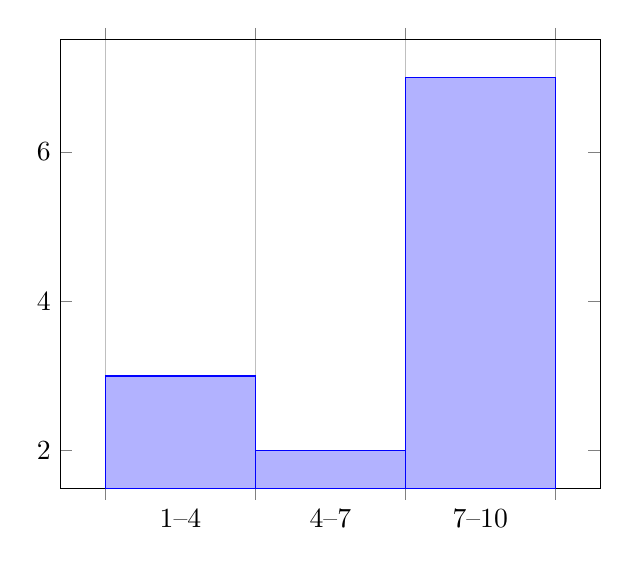
\begin{tikzpicture}
\begin{axis}[
  ybar interval,
  xticklabel=
\pgfmathprintnumber\tick--\pgfmathprintnumber\nexttick
]
	\addplot+[hist={bins=3}]
		table[row sep=\\,y index=0] {
		data\\
		1\\ 2\\ 1\\ 5\\ 4\\ 10\\ 
		7\\ 10\\ 9\\ 8\\ 9\\ 9\\ 
	};
\end{axis}
\end{tikzpicture}
\end{codeexample}
	We see that |hist={bins=3}| takes a table with one column as input. The data values fall into the range $[1,10]$ which is partitioned into~$3$ intervals (of equal lengths). Finally, the number of points falling into each of the three bins is plotted. The |xticklabel| key shows the range (note that it works only in conjunction with |x tick label as interval| which has been enabled by |ybar interval| before). We see that there are $3$ elements in the range $[1,4)$, $2$~elements in the range $[4,7)$ and finally $7$ elements in the range $[7,10]$. 
	
	The bins are half--open intervals, i.e.\ the end--point does not belong to the bin. Only the last bin contains its right end point.
\pgfplotsexpensiveexample
\begin{codeexample}[]
\begin{tikzpicture}
\begin{axis}[
  ybar interval,
  xtick=,% reset from ybar interval
  xticklabel=
    {$[\pgfmathprintnumber\tick,%
	   \pgfmathprintnumber\nexttick)$}
]
% a data file containing 8000 normally distributed
% random numbers of mean 0 and variance 1
\addplot+[hist={data=x}]
	file {plotdata/pgfplots.randn.dat};
	
\end{axis}
\end{tikzpicture}
\end{codeexample}

	The |hist| plot type can be combined with \verbpdfref{plot expression} as well: provide the usual \meta{expression} as you would for a line plot. Then, configure the value for |data=|\meta{expression} in dependence of |x|, |y|, or |z|: 
\begin{codeexample}[]
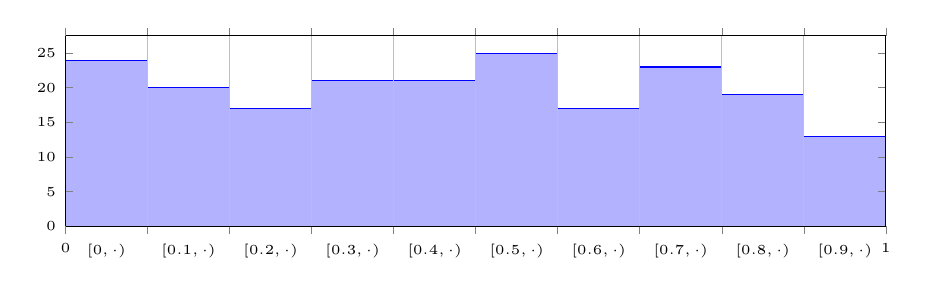
\begin{tikzpicture}
\begin{axis}[
  tiny,
  height=4cm,width=12cm,
  ybar interval,
  ymin=0,
  xmin=0,xmax=1,
  axis on top,
  extra x ticks={0,1},
  extra x tick style={
    grid=none,
    x tick label as interval=false,
    xticklabel=$\pgfmathprintnumber\tick$
  },
  xticklabel={$[\pgfmathprintnumber[fixed]\tick,\cdot)$}
]
	\addplot+[samples=200,hist] {rnd};
\end{axis}
\end{tikzpicture}
\end{codeexample}
	\noindent The example uses the |rnd| method of \pgfname\ which defines |y| to contain uniform random numbers in the range $[0,1]$. Then, it configures |hist|. Note that |hist| has the default |data=y| such that it uses the |y| coordinate as input. Note furthermore that the |x| value is effectively ignored here. The options after |\begin{axis}[...]| are mainly to scale the graphics and to insert the right limits. The |extra x ticks| method is inserted to demonstrate how to add further tick marks without affecting the overall layout. Note that the |extra x tick style| sets |x tick label as interval=false| to disable the special tick handling which is active for the rest of the plot.

	The following keys configure |hist|. If they are provided inside of \meta{options}, the common key prefix |hist/| can be omitted.

	\begin{pgfplotskey}{hist/data=\marg{expression} (initially y)}
		Tells |hist| how to get its data. 
		The common idea is to provide a mathematical \meta{expression} which depends on data supplied by the |\addplot| statement. For example, if you have |\addplot expression|, the \meta{expression} may depend upon |x|, |y| or |z|. In case of an |\addplot table| input routine, the \meta{expression} can employ |\thisrow|\marg{colname} to access the currently active table row in the designated column.
		
		It is also possible to avoid invocations of the math parser. Use \declareandlabel{hist/data value}|=|\marg{value} instead to do so. Here, \meta{value} should be of a numeric constant.

		The initial configuration employs what would usually become the final |y| coordinate as input (to be more precise, the initial value is |data value=\pgfkeysvalueof{/data point/y}|).
	\end{pgfplotskey}

	\begin{pgfplotskeylist}{%
		hist/data min=\marg{min value} (initially /pgfplots/xmin),%
		hist/data max=\marg{max value} (initially /pgfplots/xmax)}%
		Allows to provide the min/max values (the $\underline m$ and $\overline m$) values manually.

		If empty, these v (walues will be deduced from the input data range.
		
		The resulting interval will be splitted into |hist/bins| intervals.

		The initial configuration uses any provided data limits, i.e.\ the (natural) choices |hist/data min=||xmin| and |hist/data max=||xmax|.
	\end{pgfplotskeylist}

	\begin{pgfplotskey}{hist/bins=\marg{number of intervals} (initially 10)}
		Specifies the number of intervals to use.
	\end{pgfplotskey}

	\begin{pgfplotskey}{hist/intervals=\marg{true,false} (initially true)}
		If |intervals=true| (the initial configuration), |hist| will generate $N+1$ coordinates, with
		\[ \underline m = x_0 < x_1 < \dotsb < x_{N} = \overline m \]
		where $[\underline m,\overline m]$ is the data range. In this case, the data points for $x_{N-1}$ and $x_N$ will get the same value, namely the number of elements in the last bin. This is (only) useful in conjunction with |const plot| or |ybar interval|.

		If |intervals=false|, the last data point will be omitted and exactly $N$ coordinates will be generated. In this case, the right end point is not returned explicitly.
	\end{pgfplotskey}

	\begin{pgfplotskey}{hist/cumulative=\marg{true,false} (initially false)}
		Allows to compute a cumulative histogram.

		A cumulative histogram uses the sum of all previous bins and the current one as final value.

		Here is the example from above, this time with |hist/cumulative|:
		
\pgfplotsexpensiveexample
\begin{codeexample}[]
\begin{tikzpicture}
\begin{axis}[
  ybar interval,
  xtick=,% reset from ybar interval
  xticklabel=
    {$[\pgfmathprintnumber\tick,
	   \pgfmathprintnumber\nexttick)$}
]
% a data file containing 8000 normally distributed
% random numbers of mean 0 and variance 1
\addplot+[hist={
		data=x,
		cumulative}]
	file {plotdata/pgfplots.randn.dat};
	
\end{axis}
\end{tikzpicture}
\end{codeexample}
		
	\end{pgfplotskey}

	\begin{pgfplotskey}{hist/density=\marg{true,false} (initially false)}
		\textit{An extension by J\"urnjakob Dugge}
		\vskip\baselineskip
		Enables density estimation mode. If |hist/density| is active, the resulting data points will be renormalized such that the overall ``mass'' equals~$1$. 
\begin{codeexample}[]
\begin{tikzpicture}
\begin{axis}[small,ymin=0,title=\texttt{hist}]
\addplot [
	hist,
	fill=orange!75,
	draw=orange!50!black]
	table [y index=0] {plotdata/pgfplots.randn.dat};
\end{axis}
\end{tikzpicture}
%
\begin{tikzpicture}
\begin{axis}[small,ymin=0, title=\texttt{hist=density}]
\addplot [
	hist=density,
	fill=orange!75,
	draw=orange!50!black]
	table [y index=0] {plotdata/pgfplots.randn.dat};
\end{axis}
\end{tikzpicture}
\end{codeexample}


		The keys |hist/density| and |hist/cumulative| can be combined as well:
\begin{codeexample}[]
\begin{tikzpicture}
\begin{axis}[small,ymin=0, title=\texttt{hist=cumulative}]
\addplot [
	hist=cumulative,
	fill=orange!75,
	draw=orange!50!black]
	table [y index=0] {plotdata/pgfplots.randn.dat};
\end{axis}
\end{tikzpicture}
%
\begin{tikzpicture}
\begin{axis}[small,ymin=0, title=\texttt{hist=\{cumulative,density\}}]
\addplot [
	hist={cumulative,density},
	fill=orange!75,
	draw=orange!50!black]
	table [y index=0] {plotdata/pgfplots.randn.dat};
\end{axis}
\end{tikzpicture}
\end{codeexample}
	\end{pgfplotskey}

	\begin{stylekey}{/pgfplots/hist/handler (initially ybar interval)}
		Allows to change the way the generated coordinates are visualized. The |hist/handler| key is a style, so use |hist/handler/.style={const plot}| to change it.
	\end{stylekey}

	\begin{pgfplotscodekey}{hist/data filter}
		Allows to define coordinate filters, similar to the coordinate filter key |x filter| described in Section~\ref{sec:filters}. The argument |#1| is the coordinate as it has been found after processing |hist/data|. The code is supposed to assign |\pgfmathresult| to contain the result. If |\pgfmathresult| is empty afterwards, it will be skipped. Otherwise, it is supposed to contain a number.

		This filter is applied \emph{before} the histogram is computed. Note that |x filter| and |y filter| are applied \emph{after} the histogram is computed.

		Note that predefined styles like |each nth point| can also be applied to |hist/data| if
		\begin{enumerate}
			\item an asterisk `|*|' is appended to the predefined style's name and
			\item the first argument to the style is |hist/data|.
		\end{enumerate}
		For example, |each nth point*={hist/data}{2}| will skip each second input value of |hist/data| (try it out).
	\end{pgfplotscodekey}

	\begin{pgfplotsxycodekeylist}{
		/pgfplots/hist/data coord trafo,%
		/pgfplots/hist/data coord inv trafo}%
	These keys work in the same way as for |x coord trafo| and |x coord inv trafo|. They are applied to the |hist/data| value before the histogram is evaluated and after the result value is assigned, respectively.

		Note that |hist| will apply the |hist/data coord inv trafo| before it visualizes its results. Consequently, it may be necessary to assign a similar transformation to |x coord trafo| as well.

		See the documentation of |x coord trafo| for more information about custom transformations.
	\end{pgfplotsxycodekeylist}

	\begin{pgfplotskey}{hist/symbolic coords=\marg{list}}
		A style which enables |symbolic x coords| for an axis containing |hist| plots:
\begin{codeexample}[]
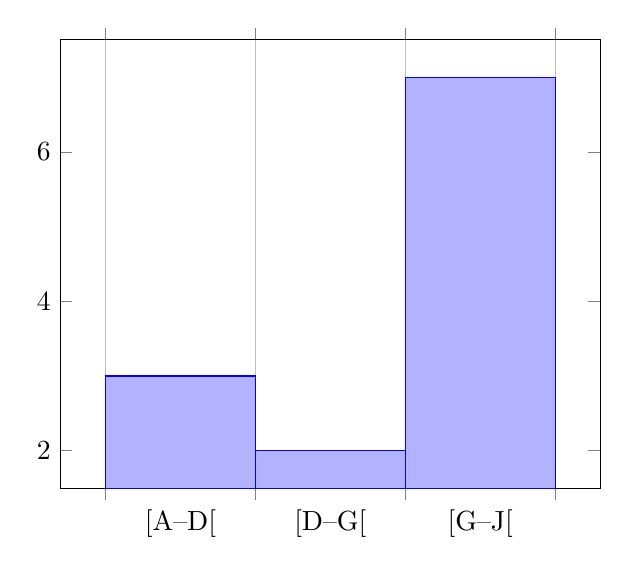
\begin{tikzpicture}
\begin{axis}[
  ybar interval,
  hist/symbolic coords={A,B,C,D,E,F,G,H,I,J},
  xticklabel={[\tick--\nexttick[},
]
    \addplot+[hist={bins=3}]
        table[row sep=\\,y index=0] {
        data\\
		A\\ B\\ A\\ D\\ F\\ J\\
		G\\ J\\ I\\ H\\ I\\ I\\
    };
\end{axis}
\end{tikzpicture}
\end{codeexample}
		The style does two things: first, it defines |hist/data coord trafo| and |hist/data coord inv trafo|, then, it calls |symbolic x coords| with the same argument.

		\paragraph{Attention}: do not use |hist/data=x| or other symbolic values as input when you have |symbolic coords|. Rather than symbolic values, you need to provide \emph{expandable} values like |\pgfkeysvalueof{/data point/x}| (which has the same effect, but directly expands to the correct value).

		Please refer to the documentation of |symbolic x coords| for further details about symbolic coordinates.
	\end{pgfplotskey}
\end{plottype}
